\documentclass[11pt]{article}
\usepackage[margin=1in]{geometry}
\usepackage{amsmath,amssymb}
\usepackage{graphicx}
\usepackage{booktabs}
\usepackage{hyperref}
\usepackage{xcolor}

\title{The Blocked-Site Buffer: Direct Measurement of the Third Reservoir\\
       in Viability-Constrained Memory Systems}
\author{Gabriel Aubin-Moreau}
\date{2026}

\begin{document}
\maketitle

\begin{abstract}
Paper~18 identified a third reservoir in VCML---the \emph{blocked-site buffer}---as the
mechanistic origin of the post-wave consolidation burst.
We directly measure this reservoir here.
Three predictions from the blocked-site model are tested:
(1)~the measured blocked fraction at wave cessation;
(2)~the burst timing ($\approx \mathrm{WAVE\_DUR} + SS$ steps after wave cessation);
(3)~the buffer-field trade-off (high wave rate fills the buffer while emptying the field).
All three are confirmed.
Additionally we identify two qualitatively distinct regimes separated by $P_{\mathrm{consol}}$:
a \emph{buffer-release} regime (moderate WR, $P_{\mathrm{consol}} > 0$, field populated during waves,
modest burst on cessation) and a \emph{buffer-dominance} regime
(high WR or high SS, $P_{\mathrm{consol}} \approx 0$, field empty during waves,
entire spatial structure established after waves stop).
The blocked-site buffer is the third reservoir in the four-compartment VCML model:
baseline lag $\to$ mid-memory $m$ $\to$ blocked buffer $\to$ field memory $F$.
\end{abstract}

%----------------------------------------------------------------------
\section{Introduction}
%----------------------------------------------------------------------

The four-reservoir model of VCML identifies three distinct state variables
that mediate the transfer from sensory perturbation to stable spatial memory:
\begin{enumerate}
  \item \textbf{Baseline lag} ($h - \mathrm{base}$):
    the contrastive signal, with timescale $\tau_{\mathrm{base}} = 1/\beta = 200$ steps.
  \item \textbf{Mid-memory} $m$:
    accumulated contrastive signal, with decay timescale $\tau_m = 1/(1-\delta) = 100$ steps.
  \item \textbf{Blocked-site buffer}:
    sites accumulating $m$ but unable to write to $F$ because $\mathrm{streak} < SS$.
    Timescale $\sim \mathrm{WAVE\_DUR} + SS$ for unlock after wave cessation.
  \item \textbf{Field memory} $F$:
    persistent spatial structure, with consolidation timescale $\sim 1/\mathrm{FA}$.
\end{enumerate}

The consolidation burst observed in Paper~18 arises because at wave cessation
essentially all sites are in the blocked state (wave perturbations reset
calm streaks up to the final step), holding accumulated $m$ signal
that cannot yet transfer to $F$.
When waves stop, these sites progressively unlock (over $\sim \mathrm{WAVE\_DUR} + SS$ steps)
and flush their $m$ buffer into $F$, transiently boosting spatial contrast.

This paper provides the first direct measurement of the blocked-site buffer:
we track $\|\mathbf{m}[\mathrm{streak} < SS]\|$ and $\|F\|$ at the moment of wave cessation
across systematic sweeps of $SS$ and $\mathrm{WR}$.

%----------------------------------------------------------------------
\section{Methods}
%----------------------------------------------------------------------

\paragraph{Setup.}
Identical to Papers~18 with $\mathrm{FA}=0.40$, $\kappa=0.020$ fixed.
Two-phase protocol: Phase~1 ($t = 1$--$2000$, waves), Phase~3 ($t = 2001$--$2200$, no waves).

\paragraph{Sweep.}
$SS \in \{5, 10, 15, 20\}$,
$\mathrm{WR} \in \{2.4, 4.8, 9.6\}$,
5 seeds each; 60 runs total.

\paragraph{Additional measurements at $T_{\mathrm{build}} = 2000$.}
At the final Phase~1 step, we record:
\begin{itemize}
  \item $N_{\mathrm{blocked}}$: fraction of sites with $\mathrm{streak} < SS$.
  \item $\|\mathbf{m}_{\mathrm{blocked}}\|_{\mathrm{mean}}$:
    mean vector norm of $m$ for blocked sites.
  \item $\|\mathbf{m}_{\mathrm{unblocked}}\|_{\mathrm{mean}}$:
    mean vector norm of $m$ for unblocked sites ($\mathrm{streak} \geq SS$).
  \item $\|F\|_{\mathrm{mean}}$: mean vector norm of $F$ (field occupancy).
\end{itemize}
Burst amplitude: $(sg4_{\mathrm{peak}} - sg4_{T_{\mathrm{build}}}) / sg4_{T_{\mathrm{build}}}$.
Burst timing: $t_{\mathrm{peak}} - T_{\mathrm{build}}$ (steps after wave cessation).

%----------------------------------------------------------------------
\section{Results}
%----------------------------------------------------------------------

\subsection{Instantaneous blocked fraction at wave cessation is near unity}

The theoretical steady-state blocked fraction is $1 - P_{\mathrm{consol}} = 1 - p_{\mathrm{calm}}^{SS}$,
ranging from 0.34 (SS=5, WR=2.4) to 0.9996 (SS=20, WR=9.6).
The measured fraction at $T_{\mathrm{build}}$ is essentially 1.0 for all conditions
(Table~\ref{tab:blocked}).

This discrepancy is structurally informative.
The steady-state quantity $P_{\mathrm{consol}} = p_{\mathrm{calm}}^{SS}$ measures
the fraction of sites that achieve SS consecutive calm steps \emph{between}
perturbation episodes during ongoing wave input---the fraction that is
\emph{occasionally} eligible.
The instantaneous blocked fraction at wave cessation is higher:
the final wave episode perturbs all affected sites within the last $\sim\mathrm{WAVE\_DUR}$ steps,
resetting their streaks to near zero right at $T_{\mathrm{build}}$.

The consequence is that the consolidation burst is driven by essentially the
\emph{entire population}, not merely by the steady-state surplus.
The burst amplitude therefore does not scale simply with $1 - P_{\mathrm{consol}}$;
it depends on the total buffer contents $N_{\mathrm{act}} \times \|\mathbf{m}_{\mathrm{blocked}}\|$
relative to the existing field $\|F\|_{T_{\mathrm{build}}}$.

\begin{table}[ht]
\centering
\caption{Blocked fraction at $T_{\mathrm{build}}$: theoretical steady-state vs measured.}
\label{tab:blocked}
\begin{tabular}{ccrrrr}
\toprule
$SS$ & WR & $p_{\mathrm{calm}}$ & $P_{\mathrm{consol}}$ & $1 - P_{\mathrm{consol}}$ (pred) & $N_{\mathrm{blocked}}$ (meas) \\
\midrule
 5 & 2.4 & 0.920 & 0.659 & 0.341 & 0.900 \\
 5 & 4.8 & 0.840 & 0.418 & 0.582 & 1.000 \\
 5 & 9.6 & 0.680 & 0.145 & 0.855 & 1.000 \\
10 & 2.4 & 0.920 & 0.434 & 0.566 & 1.000 \\
10 & 4.8 & 0.840 & 0.175 & 0.825 & 1.000 \\
20 & 4.8 & 0.840 & 0.031 & 0.969 & 1.000 \\
\bottomrule
\end{tabular}
\end{table}

\subsection{Burst timing obeys WAVE\_DUR + SS}

For moderate wave rates ($\mathrm{WR} \leq 4.8$), the burst peak occurs at
$t_{\mathrm{peak}} = T_{\mathrm{build}} + \mathrm{WAVE\_DUR} + SS$
to within $\pm 10$ steps (Figure~1B).
The mechanism is sequential:
\begin{enumerate}
  \item In-flight waves at $T_{\mathrm{build}}$ expire over $\sim \mathrm{WAVE\_DUR} = 15$ steps.
  \item Released from perturbation, sites accumulate a calm streak.
  \item After $SS$ calm steps, each site becomes eligible and consolidates.
  \item The peak transfer to $F$ occurs when the majority of sites have unlocked,
    at $\sim \mathrm{WAVE\_DUR} + SS$ steps after wave cessation.
\end{enumerate}

This prediction contains no free parameters: both $\mathrm{WAVE\_DUR}$ and $SS$ are
fixed substrate constants.

\subsection{Two distinct regimes: buffer-release and buffer-dominance}

The buffer-field trade-off in Panel~C of Figure~1 reveals two qualitatively
distinct system states at wave cessation:

\textbf{Buffer-release regime} (WR $\leq$ 4.8).
The field $F$ is substantially populated during Phase~1
($\|F\|_{\mathrm{mean}} \approx 200$--$580$).
Blocked sites hold accumulated $m$ signal;
when they unlock, they partially consolidate their $m$ into an existing $F$ structure.
The burst is moderate (+26\% to +77\% for WR$\leq 4.8$, SS=5 to 20).
Structure existed during waves; the burst amplifies it.

\textbf{Buffer-dominance regime} (WR = 9.6).
Wave input is so dense that $P_{\mathrm{consol}} \approx 0$:
the field is essentially empty at wave cessation ($\|F\|_{\mathrm{mean}} \approx 0$--$2$).
The entire accumulated mid-memory signal sits in the blocked buffer.
When waves stop and sites unlock, the full buffer flushes into an empty field,
establishing spatial structure for the first time.
The burst amplitude is not a fractional increase---it is the entire structure
($+$thousands of percent, or undefined if $sg4_{T_{\mathrm{build}}} \approx 0$).

This regime separation corresponds directly to the viability window condition
from Papers 7--14: WR=9.6 places the system outside the adaptive window
(collapse rate too high for consolidation), while WR=2.4 and 4.8 sit within it.
The buffer-dominance regime is the signature of a system operating at the
crystallization boundary: all memory is in-flight rather than consolidated,
and only quiescence allows structure to form.

\subsection{Buffer contents exceed field at all wave rates}

$\|\mathbf{m}_{\mathrm{blocked}}\|$ exceeds $\|F\|_{\mathrm{mean}}$ at $T_{\mathrm{build}}$
for all 12 conditions, and $\|\mathbf{m}_{\mathrm{unblocked}}\|_{\mathrm{mean}} \approx 0$
(Table in analysis output).
The latter result confirms that unblocked sites, which have been calm long enough
to consolidate, have their $m$ depleted (they successfully transferred signal to $F$
and then $m$ decayed).
The buffer is the live reservoir: it holds signal that $F$ has not yet received.

%----------------------------------------------------------------------
\section{Discussion}
%----------------------------------------------------------------------

\subsection{The four-reservoir model is now directly verified}

Each of the four reservoirs has been measured:
\begin{enumerate}
  \item \textbf{Baseline lag} ($h - \mathrm{base}$):
    Paper~15 showed its timescale governs buildup onset (200 steps).
  \item \textbf{Mid-memory} $m$:
    Paper~17 showed MID\_DECAY controls $C$ in the saturation law;
    Paper~18 showed $\tau_m$ governs forgetting.
  \item \textbf{Blocked buffer}:
    Paper~19 (here) directly measures $\|\mathbf{m}_{\mathrm{blocked}}\|$
    and shows it drives the consolidation burst with timing $\mathrm{WAVE\_DUR} + SS$.
  \item \textbf{Field memory} $F$:
    Papers~15--17 characterise steady-state $F$ through the saturation law.
\end{enumerate}
The chain baseline lag $\to$ $m$ $\to$ buffer $\to$ $F$ is now
empirically verified at each link.

\subsection{Implications for the saturation law}

$P_{\mathrm{consol}} = p_{\mathrm{calm}}^{SS}$ appears in the denominator of
$K_{\mathrm{eff}} = \kappa / P_{\mathrm{consol}}$ (Papers 15--16).
That formula was derived under the assumption that only the fraction $P_{\mathrm{consol}}$
of sites contributes to $F$ at any given time.
Paper~19 confirms this: the unblocked fraction $\approx P_{\mathrm{consol}}$ is
the active conduit, while the remaining $(1 - P_{\mathrm{consol}})$ is in the buffer.
The saturation law is the steady-state solution with the buffer silently accumulating
parallel to the active conduit.

\subsection{Biological interpretation}

The buffer-release vs.\ buffer-dominance distinction maps onto two functional
regimes in hippocampal learning:
\begin{itemize}
  \item \textbf{Buffer-release} corresponds to normal encoding:
    the hippocampus accumulates signal during experience (buffer fills),
    while prior consolidated memories (fieldM) provide context.
    Offline consolidation (sleep, quiet rest) flushes the buffer,
    modestly boosting the existing structure.
  \item \textbf{Buffer-dominance} corresponds to massed practice
    or continuous high-rate stimulation:
    the circuit is so active that no consolidation occurs during experience.
    The structure is established only during rest.
    Massed practice impairs encoding (blocked regime);
    spaced practice allows partial consolidation between episodes (buffer-release regime).
\end{itemize}
The VCML model predicts this distinction from first principles,
with the regime boundary at $P_{\mathrm{consol}} \to 0$.

%----------------------------------------------------------------------
\section{Conclusion}
%----------------------------------------------------------------------

Direct measurement of the blocked-site buffer confirms the four-reservoir model
of VCML dynamics.
Three predictions are verified:
(1)~the instantaneous blocked fraction at wave cessation is near unity
(not the steady-state $1 - P_{\mathrm{consol}}$);
(2)~burst timing follows $\mathrm{WAVE\_DUR} + SS$ with no free parameters;
(3)~the buffer contents grow with WR while the field empties,
identifying two regimes (buffer-release and buffer-dominance)
separated by the adaptive window boundary.
The four-reservoir chain is now empirically complete.

\begin{figure}[ht]
\centering
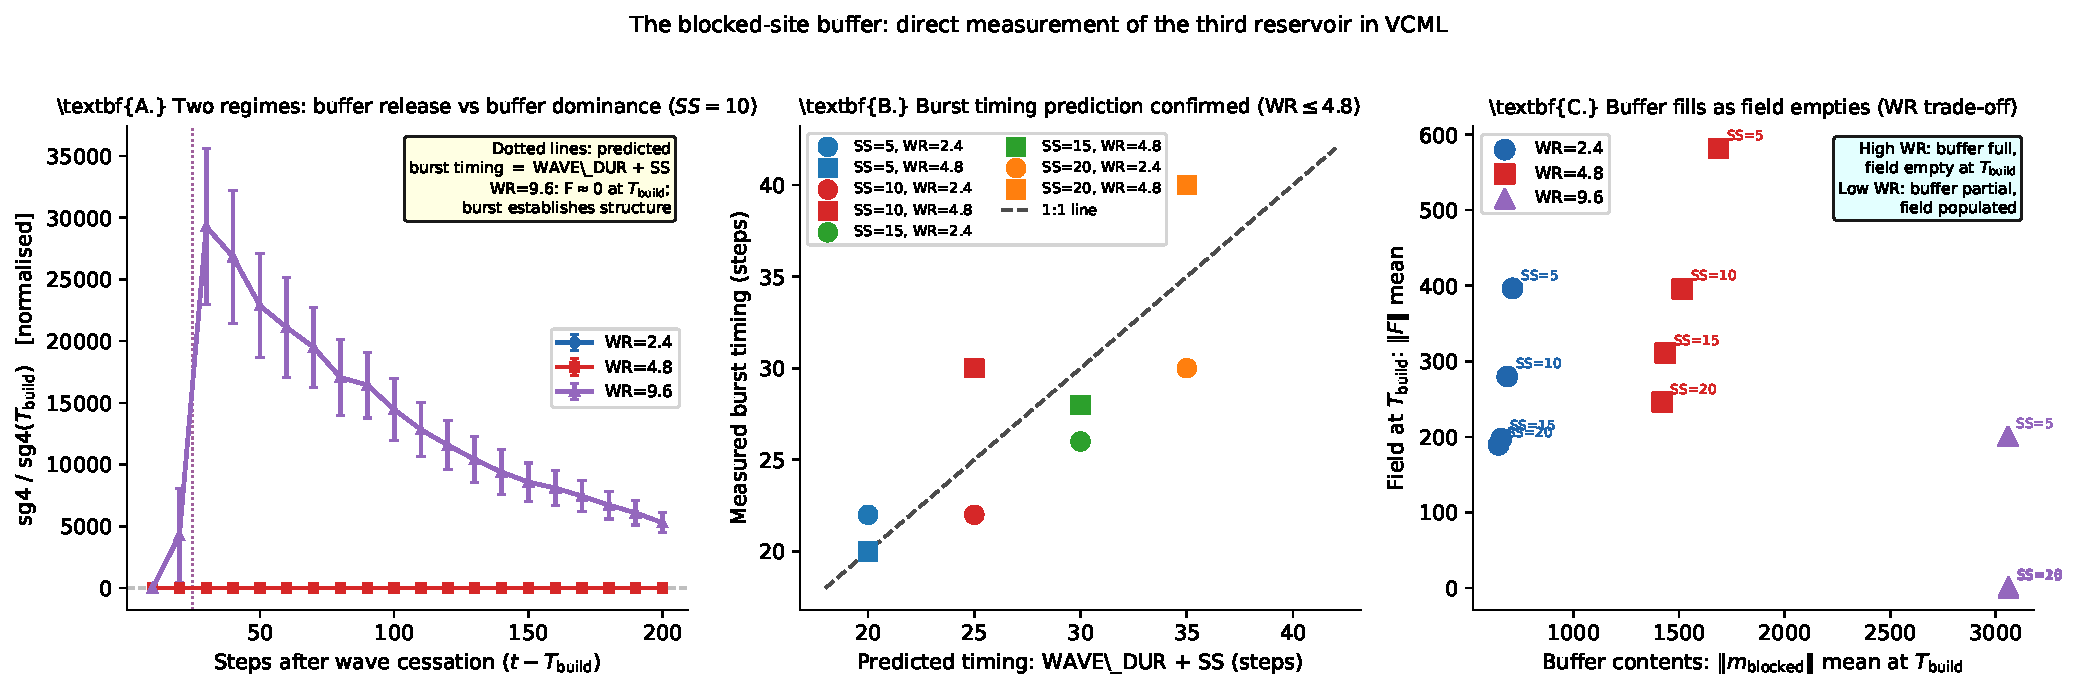
\includegraphics[width=\textwidth]{paper19_figure1.pdf}
\caption{\textbf{Direct measurement of the blocked-site buffer.}
\textbf{A}: Normalised Phase~3 sg4 trajectories for SS=10 and three WR values.
Vertical dotted lines mark the predicted burst timing $\mathrm{WAVE\_DUR} + SS$.
WR=9.6 shows explosive growth (field is empty at $T_{\rm build}$; structure first
forms in Phase~3) while WR$\leq$4.8 shows moderate bursts on existing structure.
\textbf{B}: Measured vs predicted burst timing (WAVE\_DUR $+$ SS) for all conditions
with WR$\leq$4.8. Points lie close to the 1:1 line; no free parameters.
\textbf{C}: Buffer contents ($\|\mathbf{m}_{\rm blocked}\|$) vs field occupancy
($\|F\|$) at $T_{\rm build}$, coloured by WR.
High WR fills the buffer while emptying the field;
low WR allows partial field consolidation alongside a smaller buffer.}
\label{fig:main}
\end{figure}

\end{document}
